%%%%%%%%%%%%%%%%%%%%%%%%%
% Dokumentinformationen %
%%%%%%%%%%%%%%%%%%%%%%%%%
\newcommand{\titleinfo}{Integraltransformationen - Formelsammlung}
\newcommand{\authorinfo}{Braun \& Co, J.Rast}
\newcommand{\versioninfo}{$Revision: 1 $ - powered by \LaTeX}

%%%%%%%%%%%%%%%%%%%%%%%%%%%%%%%%%%%%%%%%%%%%%
% Standard projektübergreifender Header für
% - Makros 
% - Farben
% - Mathematische Operatoren
%
% DORT NUR ERGÄNZEN, NICHTS LÖSCHEN
%%%%%%%%%%%%%%%%%%%%%%%%%%%%%%%%%%%%%%%%%%%%%
% Genereller Header
\documentclass[10pt,twoside,a4paper,fleqn]{article}
% Dateiencoding
\usepackage[utf8]{inputenc}
% Seitenränder
\usepackage[left=1cm,right=1cm,top=1cm,bottom=1cm,includeheadfoot]{geometry}
% Sprachpaket
\usepackage[ngerman]{babel,varioref}

% Pakete
\usepackage{amssymb,amsmath,fancybox,graphicx,lastpage,wrapfig,fancyhdr,hyperref,verbatim,floatflt,multicol,multirow,rotating,pdflscape,array,longtable,listings}

% Zum Bilder einfach in Tabellen einfügen (valign=t)
\usepackage[export]{adjustbox}

%%%%%%%%%%%%%%%%%%%%
% Generelle Makros %
%%%%%%%%%%%%%%%%%%%%
\newcommand{\skript}[1]{$_{\textcolor{red}{\mbox{\small{Skript S.#1}}}}$}
\newcommand{\verweis}[2]{\small{(siehe auch \ref{#1}, #2 (S. \pageref{#1}))}}
\newcommand{\verweiskurz}[1]{(\small{siehe \ref{#1}\normalsize)}}
\newcommand{\subsubadd}[1]{\textcolor{black}{\mbox{#1}}}
\newcommand{\formelbuch}[1]{$_{\textcolor{red}{\mbox{\small{S#1}}}}$}

\newcommand{\kuchling}[1]{$_{\textcolor{red}{\mbox{\small{Kuchling #1}}}}$}
\newcommand{\stoecker}[1]{$_{\textcolor{orange}{\mbox{\small{Stöcker #1}}}}$}
\newcommand{\sachs}[1]{$_{\textcolor{blue}{\mbox{\small{Sachs S. #1}}}}$}
\newcommand{\hartl}[1]{$_{\textcolor{green}{\mbox{\small{Hartl S. #1}}}}$}

\newcommand{\schaum}[1]{\tiny Schaum S. #1}

\newcommand{\skriptsection}[2]{\section{#1 {\tiny Skript S. #2}}}
\newcommand{\skriptsubsection}[2]{\subsection{#1 {\tiny Skript S. #2}}}
\newcommand{\skriptsubsubsection}[2]{\subsubsection{#1 {\tiny Skript S. #2}}}

\newcommand{\matlab}[1]{\footnotesize{(Matlab: \texttt{#1})}\normalsize{}}

%%%%%%%%%%
% Farben %
%%%%%%%%%%
\usepackage{xcolor}

%%%%%%%%%%%%%%%%%%%%%%%%%%%%
% Mathematische Operatoren %
%%%%%%%%%%%%%%%%%%%%%%%%%%%%
\DeclareMathOperator{\sinc}{sinc}
\DeclareMathOperator{\sgn}{sgn}
\DeclareMathOperator{\Real}{Re}
\DeclareMathOperator{\Imag}{Im}
%\DeclareMathOperator{\e}{e}
\DeclareMathOperator{\cov}{cov}
\DeclareMathOperator{\PolyGrad}{PolyGrad}

%Makro für 'd' von Integral- und Differentialgleichungen 
\newcommand*{\diff}{\mathop{}\!\mathrm{d}}


%%%%%%%%%%%%%%%%%%%%%%%%%%%
% Fouriertransformationen %
%%%%%%%%%%%%%%%%%%%%%%%%%%%
\usepackage{trfsigns, trsym}
%\unitlength1cm
% Zeitbereich -- Frequenzbereich
%\newcommand{\laplace}
%{
%\begin{picture}(1,0.5)
%\put(0.2,0.1){\circle{0.14}}\put(0.27,0.1){\line(1,0){0.5}}\put(0.77,0.1){\circle*{0.14}}
%\end{picture}
%}
% Frequenzbereich -- Zeitbereich
%\newcommand{\Laplace}
%{
%\begin{picture}(1,0.5)
%\put(0.2,0.1){\circle*{0.14}}\put(0.27,0.1){\line(1,0){0.45}}\put(0.77,0.1){\circle{0.14}}
%\end{picture}
%}


% Fouriertransformationen
\unitlength1cm
\newcommand{\FT}
{
\begin{picture}(1,0.5)
\put(0.2,0.1){\circle{0.14}}\put(0.27,0.1){\line(1,0){0.5}}\put(0.77,0.1){\circle*{0.14}}
\end{picture}
}


\newcommand{\IFT}
{
\begin{picture}(1,0.5)
\put(0.2,0.1){\circle*{0.14}}\put(0.27,0.1){\line(1,0){0.45}}\put(0.77,0.1){\circle{0.14}}
\end{picture}
}




%%%%%%%%%%%%%%%%%%%%%%%%%%%%
% Allgemeine Einstellungen %
%%%%%%%%%%%%%%%%%%%%%%%%%%%%
%PDF Info
\hypersetup{pdfauthor={\authorinfo},pdftitle={\titleinfo},colorlinks=false}
\author{\authorinfo}
\title{\titleinfo}

%%%%%%%%%%%%%%%%%%%%%%%
% Kopf- und Fusszeile %
%%%%%%%%%%%%%%%%%%%%%%%
\pagestyle{fancy}
\fancyhf{}
%Linien oben und unten
\renewcommand{\headrulewidth}{0.5pt} 
\renewcommand{\footrulewidth}{0.5pt}

\fancyhead[L]{\titleinfo{ }\tiny{(\versioninfo)}}
%Kopfzeile rechts bzw. aussen
\fancyhead[R]{Seite \thepage { }von \pageref{LastPage}}
%Fusszeile links bzw. innen
\fancyfoot[L]{\footnotesize{\authorinfo}}
%Fusszeile rechts bzw. ausen
\fancyfoot[R]{\footnotesize{\today}}
%Lizenz CC-BY-NC-SA
% Headerfile für die Einbindung einer Lizenzgrafik in den Footer
% Verwendung: \lizenz{cc-by-nc-sa}{small}
\newcommand{\lizenz}[2]
{
\fancyfoot[C]{
  \includegraphics[width=1.6cm]{./header/lizenzen/#1/#2.png}
}
}
\lizenz{cc-by-nc-sa}{small}
%Einrücken verhindern versuchen
\setlength{\parindent}{0pt}

% Zeilenhöhe Tabellen:
\newcommand{\arraystretchOriginal}{1.5}
\renewcommand{\arraystretch}{\arraystretchOriginal}



% Möglichst keine Ergänzungen hier, sondern in header.tex
\begin{document}
%%%%%%%%%%%%%%%%%%%%%%%%%%%%%%%%%%%%%%%%%%%%%%%%%%%%%%%%%%%%%%%%%%%%%%%%%%%%%%%%%%%%%%%%%%%%%%%%
%%%%%%%%%%%%%%%%%%%%%%%%%%%%%%%%%%%%%%%%%%%%%%%%%%%%%%%%%%%%%%%%%%%%%%%%%%%%%%%%%%%%%%%%%%%%%%%%

% Einleitung
\section{Varianten der Integraltransformationen}
\begin{tabular}{|l||l|l|}
\hline & & \\
\textbf{Signalart}
	& diskret
	& kontinuierlich \\
\hline \hline & & \\
periodisch
	& Diskrete Fourier-Transformation
	& Fourierreihe \\
\hline & & \\
impulsförmig
	& ``Fourierreihe mit $T = Impulsdauer$''
	& Fourierintegral \\
\hline & & \\
kausal
	& Z-Transformation
	& Laplace-Transformation \\
\hline
\end{tabular}

% Signale und Systeme
\section{Signale und Systeme}
  	\renewcommand{\arraystretch}{1.5}
	\begin{tabular}{|l|l|}
    	\hline
    	\textbf{Linearität} & \textbf{Zeitinvarianz}\\
    	\hline
    	$S(x1+x2)=S(x1)+S(x2)$ & $S(x(t-t_0)=S(x)\cdot x(t-t_0)$ \\
    	$S(c\cdot x)=c\cdot S(x)$ & \\
		\hline    
    \end{tabular}
  	\renewcommand{\arraystretch}{1}
  	
	\subsection{Lineare Systeme}
		\textbf{Basissignale}
		\begin{list}{$\bullet$}{\setlength{\itemsep}{0cm} \setlength{\parsep}{0cm} \setlength{\topsep}{0cm}} 
          \item Lineare Systeme sind durch die Antworten auf die
          Basissignale bestimmt.
          \item Basissignale müssen linear unabhängig voneinander sein, d.h. ein
		Basissignal darf nicht durch \textbf{Linearkombination} anderer Basissignale
		darstellbar sein          
		  \item Alle möglichen Eingangs-Funktionen müssen durch eine Linearkombination der
		Basissignale dargestellt werden können. $\Rightarrow$ \textbf{Periode des Eingangssignals =	Anzahl Basissignale}
        \end{list}
        \vspace{.2cm}
		\textbf{Berechnung der Systemantwort aufgrund der Basissignale und der
		Anregung}\\
		1. Eingangssignal $x$ als Linearkombination der Basisvektoren darstellen
		$\Rightarrow$ lineares Gleichungssystem\\
		$\Rightarrow x=r\cdot a + s\cdot b + t\cdot c\qquad$ ($x=$
		Eingangssignal; $a,b,c=$ Basisvektoren; $r,s,t=$
		Linearkombinationsparameter)\\ 
		2. Systemantwort $y=r\cdot S(a) + s\cdot S(b) + t\cdot S(c); \qquad (S(a)=$
		Systemantwort der Basis $a$)
	
	\subsection{Lineare zeitinvariante Systeme (LTI-Systeme)}
		LTI-Systeme sind durch ihre Impulsantwort $h$ vollständig bestimmt\\ \\
		\textbf{Berechnung der Systemantwort von diskreten LTI-Systemen}\\
		$\; y=x*h \qquad$ ($y=$ Systemantwort; $x=$ Eingangssignal; $h=$
		Impulsantwort)\\
		
		\textbf{Berechnung der Systemantwort von kontinuierlichen LTI-Systemen}\\
		\begin{tabular}{ll}
			\parbox{8cm}{
			$$s_2(t) = h(t) * s_1(t) \FT S_2(s) = H(s) S_1(s)$$
			$$h(t) \FT H(s)$$}
			& \parbox{8cm}{
			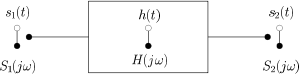
\includegraphics[width=5cm]{../SigSys1/bilder/utf-theorie.png}}\\
		\end{tabular}	
		
	\subsection{Faltung}
		\begin{tabular}{ll}
	        $\boxed{y=x*h=h*x}$&$h=$Impulsantwort des Systems\\ & \\
	   		\textbf{diskret}& \textbf{kontinuierlich}\\
	   		$\boxed{y(i)=\sum\limits_{k=-\infty}^{\infty}x(k)\cdot
	   		h(i-k)=\sum\limits_{k=-\infty}^{\infty}x(i-k)\cdot h(k)}$&
	   		$\boxed{y(t)=\int\limits_{-\infty}^{\infty}x(\tau)\cdot
	   		h(t-\tau)\cdot d\tau=\int\limits_{-\infty}^{\infty}x(t-\tau)\cdot
	   		h(\tau)\cdot d\tau}$\\ & \\
	   		grafische Interpretation: & grafische Interpretation:\\
	   		\parbox{8cm}{1. einfacheres Signal an der Y-Achse spiegeln\\
	   					2. Verschiebung um  $i$ nach rechts\\
	   					3. Skalarprodukt der beiden Signale bilden}&
			\parbox{8cm}{1. einfacheres Signal an der Y-Achse spiegeln\\
			 			2. Verschiebung um $t$ nach rechts\\
			 			3. Multiplikation und Integration der beiden Signale}		
        \end{tabular}
	
\newpage

% Diskrete Fourier Transformation
%\section{Diskrete Fourier Transformation (DFT)}
	$$\boxed{s(h)=\sum_{k=0}^{N-1}\hat c_k e^{jhk\frac{2\pi}{N}}=\sum_{k=0}^{N-1}
	\left[ \hat{a}_k \cos\left(hk \frac{2 \pi}{N}\right)+\hat{b}_k \sin\left(hk
	\frac{2 \pi}{N}\right) \right]} \qquad N=\text{Periodenanzahl}$$\\
	$$\hat{c}_k=\frac{1}{N}\sum_{h=0}^{N-1}s(h)
	e^{-jhk\frac{2\pi}{N}}=\hat{a}_k-j\hat{b}_k \qquad \hat{a}_k=\frac{1}{N}
	\sum_{h=0}^{N-1}s(h) \cos\left(hk \frac{2 \pi}{N}\right)=Re(\hat{c}_k) \qquad
	\hat{b}_k=\frac{1}{N} \sum_{h=0}^{N-1}s(h) \sin\left(hk \frac{2
	\pi}{N}\right)=-Im(\hat{c}_k)$$\\	

	\subsection{Berechnung mit Matrizen}
		\textbf{Transformation}\\
		1. Periode $N$ des Signalvektors $\vec{s}=
		\begin{bmatrix}
		s(0) \\
		s(1) \\
		s(N-1)\\
		\end{bmatrix}$ bestimmen\\ \\
		2. Einheitswurzel $w$ berechnen: $w=e^{j\frac{2 \pi}{N}}$\\ \\
		3. Matrix $W$ berechnen: $W=
		\begin{bmatrix}
		w^0 & w^0 & w^0 & \ldots & w^0\\
		w^0 & w^1 & w^2 & \ldots & w^{N-1}\\
		w^0 & w^2 & w^4 & \ldots & w^{2(N-1)}\\
		\ldots & \ldots & \ldots & \ldots & \ldots\\
		w^0 & w^{N-1} & w^{2(N-1)} & \ldots & w^{(N-1)(N-1)}                        
		\end{bmatrix}$\\ \\
		4. Matrix $V$ berechnen: $V=W^*$ (konj. komplex)\\ \\
		5. Koeffizienten bzw. Fouriertransformierte $\vec{c}$ berechnen:
		$\vec{c}=\frac{1}{N}V\vec{s}$\\

		\begin{minipage}{13cm}
			\textbf{Rücktransformation}\\
			1. Matrix $W$ (wie bei der Transformation beschrieben) berechnen \\
			2. Signalvektor $\vec{s}$ berechnen: $\vec{s}=W\vec{c}$	
			\subsection{Matrizenmultiplikation}
			\begin{tabular}{ll}
				$\frac14
				\begin{bmatrix}
				    6 & -1 & 4 \\
				    3 & 2 & -2 \\
				    0 & -3 & -1
				\end{bmatrix}
				\cdot
				\begin{bmatrix}
					1 \\
				    4 \\
				    3 
				\end{bmatrix}
				=
				\frac14
				\begin{bmatrix}
					6 \cdot 1 + (-1) \cdot 4 + 4 \cdot 3\\
					3 \cdot 1 + 2 \cdot  4 + (-2) \cdot 3\\
					0 \cdot 1 + (-3) \cdot 4 + (-1) \cdot 3  
				\end{bmatrix}
				=
				\frac14
				\begin{bmatrix}
				    14\\
				    5\\
				    -15
				\end{bmatrix}
				=
				\begin{bmatrix}
		        	3.5\\
		        	1.25\\
		        	-3.75
		        \end{bmatrix}$
		    \end{tabular}		
        \end{minipage}
		\begin{minipage}[c]{5cm}
        	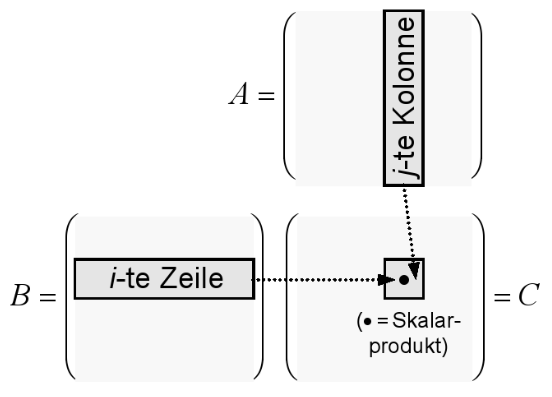
\includegraphics[width=5cm]{../IntTra/bilder/matrix.png}
        \end{minipage}
		
	\subsection{Einige W-Matrizen}
		\begin{tabular}{l l l l}
        N = 2 & N = 3 & N = 4 & N = 6\\
		$\begin{bmatrix}
		1 & 1\\
		1 & -1\\              
		\end{bmatrix}$ &
		$\begin{bmatrix}
		1 & 1 & 1\\
		1 & -\frac{1}{2}+j\frac{\sqrt{3}}{2} & -\frac{1}{2}-j\frac{\sqrt{3}}{2}\\
		1 & -\frac{1}{2}-j\frac{\sqrt{3}}{2} & -\frac{1}{2}+j\frac{\sqrt{3}}{2}\\
		\end{bmatrix}$ &
		$\begin{bmatrix}
		1 & 1 & 1 & 1 \\
		1 & j & -1 & -j\\
		1 & -1 & 1 & -1\\
		1 & -j & -1 & j\\                   
		\end{bmatrix}$ &
		$\begin{bmatrix}
		1 & 1 & 1 & 1 & 1 & 1\\
		1 & \frac{1}{2}+j\frac{\sqrt{3}}{2} & -\frac{1}{2}+j\frac{\sqrt{3}}{2} & -1
		& -\frac{1}{2}-j\frac{\sqrt{3}}{2} & \frac{1}{2}-j\frac{\sqrt{3}}{2}\\
		1 & -\frac{1}{2}+j\frac{\sqrt{3}}{2} & -\frac{1}{2}-j\frac{\sqrt{3}}{2} & 1
		& -\frac{1}{2}+j\frac{\sqrt{3}}{2} & -\frac{1}{2}-j\frac{\sqrt{3}}{2}\\
		1 & -1 & 1 & -1 & 1 & -1\\
		1 & -\frac{1}{2}-j\frac{\sqrt{3}}{2} & -\frac{1}{2}+j\frac{\sqrt{3}}{2} & 1
		& -\frac{1}{2}-j\frac{\sqrt{3}}{2} & -\frac{1}{2}+j\frac{\sqrt{3}}{2}\\ 
		1 & \frac{1}{2}-j\frac{\sqrt{3}}{2} & -\frac{1}{2}-j\frac{\sqrt{3}}{2} & -1
		& -\frac{1}{2}+j\frac{\sqrt{3}}{2} & \frac{1}{2}+j\frac{\sqrt{3}}{2}\\ 
		\end{bmatrix}$
		\end{tabular}

		\begin{tabular}{l }
        N = 8\\
 		$\begin{bmatrix}
		1 & 1 & 1 & 1 & 1 & 1 & 1 & 1\\ 
		1 & \frac{\sqrt{2}}{2}+\frac{\sqrt{2}}{2}j & j &
		-\frac{\sqrt{2}}{2}+\frac{\sqrt{2}}{2}j & -1 & 
		-\frac{\sqrt{2}}{2}-\frac{\sqrt{2}}{2}j & -j & 
		\frac{\sqrt{2}}{2}-\frac{\sqrt{2}}{2}j\\
		1 & j & -1 & -j & 1 & j & -1 & -j\\
		1 &	-\frac{\sqrt{2}}{2}+\frac{\sqrt{2}}{2}j & -j & 
		\frac{\sqrt{2}}{2}+\frac{\sqrt{2}}{2}j & -1 & 
		\frac{\sqrt{2}}{2}-\frac{\sqrt{2}}{2}j & j &
		-\frac{\sqrt{2}}{2}-\frac{\sqrt{2}}{2}j\\
		1 & -1 & 1 & -1 & 1 & -1 & 1 & -1\\
		1 &	-\frac{\sqrt{2}}{2}-\frac{\sqrt{2}}{2}j & j &
		\frac{\sqrt{2}}{2}-\frac{\sqrt{2}}{2}j & -1 &
		\frac{\sqrt{2}}{2}+\frac{\sqrt{2}}{2}j & -j &
		-\frac{\sqrt{2}}{2}+\frac{\sqrt{2}}{2}j\\
		1 & -j & -1 & j & 1 & -j & -1 & j\\
		1 &	\frac{\sqrt{2}}{2}-\frac{\sqrt{2}}{2}j & -j & 
		-\frac{\sqrt{2}}{2}-\frac{\sqrt{2}}{2}j & -1 &
		-\frac{\sqrt{2}}{2}+\frac{\sqrt{2}}{2}j & j &
		\frac{\sqrt{2}}{2}+\frac{\sqrt{2}}{2}j
		\end{bmatrix}$
		\end{tabular}


	
	
	
	
%\newpage

% Fourierreihe
\section{Fourierreihe}
  	$$\boxed{f(t) = \sum\limits_{k = -\infty}^{\infty} c_k \cdot e^{j k \omega_1
  	t}}= \boxed{\sum\limits_{k = 0}^{\infty} \left(c_k \cdot e^{j k \omega_1
  	t} + \overline{c_k} \cdot e^{-j k \omega_1t}\right)}$$
  	$$\boxed{f(t) = \frac{a_0}{2} + \sum\limits_{k=1}^{\infty} \left[a_k \cos(k
  	\omega_1 t) + b_k \sin(k \omega_1 t)\right]}=\boxed{\frac{A_0}{2} +
  	\sum\limits_{k=1}^{\infty} A_k \cos(k \omega_1 t + \varphi_k)} \quad k\in
  	\mathbb{Z}, \quad \omega_1=\frac{2 \pi}{T}=2 \pi f$$	
	
	$$\boxed{c_k=\overline{c_{-k}}=\frac{1}{T}\int_0^T{f(t)\cdot
	e^{-jk\omega_1
	t}dt} \; ; \; c_0 \neq a_0} \qquad \boxed{a_0 = \frac{2}{T}\int\limits_0^{T}
	f(t)dt, \quad a_k = \frac{2}{T}\int\limits_0^{T} f(t)\cos(k \omega_1 t) dt, \quad b_k =
	\frac{2}{T}\int\limits_0^{T} f(t)\sin(k \omega_1 t) dt}$$

	$a_0$, $c_0$, $A_0$ sind \textit{Konstanten}, $\omega_1$ ist die
	\textit{Grundkreisfrequenz}, $a_k$ und $b_k$ sind die \textit{reellen
	Koeffizienten}, $c_k$ ist der \textit{komplexe Koeffizient}, $A_k$ ist die
	\textit{Amplitude} und $\varphi_k$ ist die \textit{Phase}.\\
	\fbox{
	\begin{tabular}{p{9cm}p{9cm}}
		$a_k = c_k + \bar{c_k} = 2\Real(c_k) = A_k \cos(\varphi_k)$ &
		$b_k = j(c_k + \bar{c_k}) = -2\Imag(c_k) = -A_k \sin(\varphi_k)$ \\ \\
		$c_k = \frac{a_k-jb_k}{2} = \frac{A_k}{2} e^{j\varphi_k} = \frac1T
		F(j k \omega)$ &
		$c_{-k} = \overline{c_k} = \frac{a_k+jb_k}{2} = \frac{A_k}{2} e^{-j\varphi_k}$ \\ \\
		$A_k = 2|c_k| = \sqrt{a_k^2+b_k^2}$ & $\varphi_k =  \arg(c_k)$\\
	\end{tabular}}\\

	\textbf{Berechnung von $\varphi_k$ aus $a_k$ und $b_k$}\\
	\begin{tabular}{p{4cm}p{4cm}p{3cm}p{3.5cm}}
		$a_k> 0:$ & $\varphi_k = -\arctan(\frac{b_k}{a_k})$ &
		$a_k<0:$ &	$\varphi_k = -\arctan(\frac{b_k}{a_k}) + \pi$\\
		$a_k = 0 \wedge b_k > 0:$ &	$\varphi_k = -\frac{\pi}{2}$ &
		$a_k = 0 \wedge b_k < 0:$ &	$\varphi_k = \frac{\pi}{2}$\\
		$a_k = 0 \wedge b_k = 0:$ &	$\varphi_k = \text{nicht definiert}$
	\end{tabular}

	\subsection{Symmetrie}
		\begin{tabular}{|p{4.3cm}|p{4.3cm}|p{4.4cm}|p{4.4cm}|}
         	\hline
        	\textbf{gerade Funktion} & \textbf{ungerade Funktion} &
        	\textbf{Halbperiode 1} & \textbf{Halbperiode 2}\\
        	\hline
        	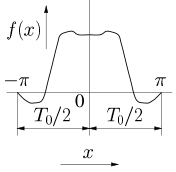
\includegraphics[width=3cm]{../IntTra/bilder/gerade_funktion.png}&
        	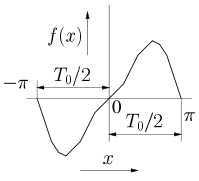
\includegraphics[width=3cm]{../IntTra/bilder/ungerade_funktion.png}&   
 			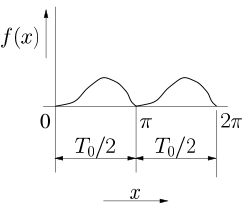
\includegraphics[width=3cm]{../IntTra/bilder/halbperiode_1.png}&   
			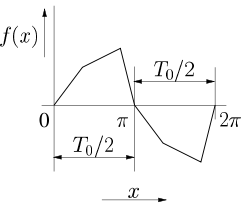
\includegraphics[width=3cm]{../IntTra/bilder/halbperiode_2.png}\\
			\hline & & & \\			
   			$f(-t)=f(t)$ & $f(-t)=-f(t)$ & $f(t)=f(t+\pi)$ & $f(t)=-f(t+\pi)$\\
   			$b_k=0$ & $a_k=0$ & $a_{2k+1}=0$ & $a_{2k}=0$\\
   			$a_k = \frac{4}{T} \int\limits_0^{\frac{T}{2}} f(t) \cdot \cos(k \omega_1
   			t) dt$ &
   			$b_k =  \frac{4}{T} \int\limits_0^{\frac{T}{2}} f(t) \cdot
			\sin(k \omega_1 t) dt$ &
			$b_{2k+1}=0$ & $b_{2k}=0$\\
			\hline
      	\end{tabular}

	\subsection{Rechtecksignale}
	$$a_k=\frac{2}{T}\int\limits_{-t_1/2}^{t_1/2}A\cos\left(\frac{2\pi k}{T}t\right)dt=
	\left .\frac{2AT}{2\pi T k}\sin \left(\frac{2\pi k}{T}t\right)\right |_{-t_1/2}^{t_1/2}=
	\frac{2A}{\pi k}\sin\left(\frac{\pi t_1}{T}k\right)$$
	F"ur Verh"altnisse $\frac{T}{ggT(t_1,T)}=n\in\mathbb{N}$ verschwinden die
	$n.$ Harmonische und deren Vielfache.\\
	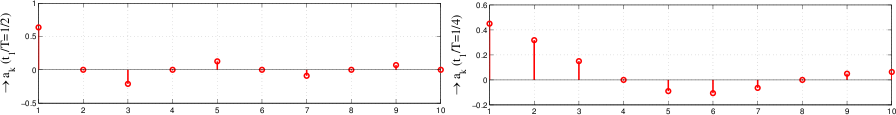
\includegraphics[width=19cm]{../IntTra/bilder/fourierreihe-rechteck.png}
\newpage
	
% Fourier-Integral / Fourier-Transformation
\section{Fourier-Integral / Fourier-Transformation}
\begin{tabular}{|ll|}
\hline
\textbf{Fouriertransformierte/Fourierintegral:} &
$F(j\omega) = \int\limits_{-\infty}^{\infty} f(t)e^{-j\omega t}dt$ \\

\textbf{Rücktransformierte:} &
$f(t) = \frac{1}{2\pi}\int\limits_{-\infty}^{\infty}F(j\omega)e^{j\omega t}d\omega$ \\

Dies ergibt das \textbf{Korespondenzpaar:} & $f(t) \laplace F(\omega)$ \\
mit der \textbf{Symetrie:} & $F(t) \laplace 2\pi \cdot f(-\omega)$ \\

$F(\omega) = R(\omega) -jX(\omega)$ wobei: ($f(t)$ reell!) &
$R(\omega) = \int\limits_{-\infty}^\infty f(t)\cdot \cos(\omega t)\,dt \quad\quad X(\omega) =
\int\limits_{-\infty}^\infty f(t)\cdot \sin(\omega t)\,dt$
\\
&$f(t)$ gerade: $X(\omega)$ verschwindet, f(t) ungerade: $R(\omega)$ verschwindet \\
\hline
\end{tabular}

Jede reelle $f(t)$ lässt sich aus Summe einer geraden und einer ungeraden Funktion beschreiben:\\
\begin{tabular}{lll}
$f(t) = f_e(t) + f_o(t)$ mit & $f_e(t) = \frac{1}{2}[f(t) + f(-t)]$ & $f_o(t) = \frac{1}{2}[f(t) - f(-t)]$ \\

Also: & $R(\omega) = 2 \int\limits_0^\infty f_e(t) \cos(\omega t)\,dt$ & $X(\omega) = 2 \int\limits_0^\infty
f_o(t) \sin(\omega t)\,dt$ \\

Und: & $f_e(t) = \frac{1}{\pi}\int\limits_0^\infty R(\omega)\cos(\omega t)\,d\omega$ & 
$f_o(t) = \frac{1}{\pi}\int\limits_0^\infty X(\omega)\sin(\omega t)\,d\omega$ \\
\end{tabular}

Bei \textbf{kausalen} Funktionen gilt:\\
$f_e(t) = f_o(t) = \frac{1}{2}f(t) \quad \quad \quad
f(t) = \frac{2}{\pi}\int\limits_0^\infty R(\omega) \cos(\omega t)\,dt = \frac{2}{\pi}\int\limits_0^\infty X(\omega)
\sin(\omega t)\,dt$

\begin{tabular}{|l|l|l|}
\hline
Spektraldichte / Spektraldarstellung	& $F(\omega)$ 		& KEINE absoluten Werte für Amplitude \& Phase \\
\hline
Amplitudendichte 						& $|F(\omega)|$		& f reell $\rightarrow$ $|F(\omega)|$ symetrisch zur Ordinatenachse \\
\hline
Phasendichte							& $arg(F(\omega))$	& f reell $\rightarrow$ $arg(F(\omega))$ punktsymetrisch zum Ursprung \\
\hline
Kosinusamplitudendichte					& $R(\omega)$		& f reell $\rightarrow$ $R(\omega)$ gerade \\
\hline
Sinusamplitudendichte					& $X(\omega)$ 		& f reell $\rightarrow$ $X(\omega)$ ungerade \\
\hline
\end{tabular}


\subsection{Symmetrie}
	Es gelten die gleichen Symmetrien wie bei der Fourierreihe.
		
	\subsection{Eigenschaften}
		\begin{tabular}{|p{8cm}|p{8cm}|}
        	\hline
        	Linearität & 
        	$\alpha\cdot f(t) + \beta\cdot g(t) \laplace \alpha\cdot F(j\omega) +
        	\beta\cdot G(j\omega)$\\
        	\hline
			Zeitumkehrung (Spiegelung an der Y-Achse)&
			$f(-t) \laplace F(-j\omega) = F^*(jw)$ \\
			\hline        	
  			"Ahnlichkeit / Zeitskalierung &
  			$f(\alpha t) \laplace \frac{1}{|\alpha|}F \left (j\frac{\omega}{\alpha} \right)
  			\quad\alpha \in\mathbb{R}\setminus \{0\}$\\
  			\hline
  			Verschiebung im	Zeitbereich &
  			$f(t\pm t_0) \laplace F(j\omega)e^{\pm j\omega t_0}$\\
  			\hline
			Verschiebung im Frequenzbereich &
			$f(t)e^{\pm j\omega_0 t} \laplace F(j(\omega\mp\omega_0))$\\
			\hline
			Ableitung im Zeitbereich &
			$\frac{\partial^n f(t)}{\partial t^n} \laplace (j\omega)^n F(j\omega)$\\
			\hline
			Integration im Zeitbereich &
			$\int\limits_{-\infty}^{t}f(\tau)d\tau \laplace
			\frac{F(j\omega)}{j\omega}+F(0)\pi\delta(\omega)$\\
			\hline				
			Ableitung im Frequenzbereich &
			$t^n f(t) \laplace j^n \frac{\partial F(j\omega)}{\partial \omega^n}$\\
			\hline		
			Faltung im Zeitbereich &
			$f(t) \ast g(t) = \int\limits_{-\infty}^{\infty} f(\tau)g(t-\tau)d\tau \laplace
			F(j\omega) \cdot G(j\omega)$\\
			\hline
			Faltung im Frequenzbereich &
			$f(t) \cdot g(t) \laplace \frac{1}{2\pi}F(j\omega) \ast G(j\omega)$\\
			\hline
			Vertauschungssatz (Dualität) &
			$f(t) \laplace F(j\omega)\nonumber$ \\
 			& $F(t) \laplace 2\pi \cdot f(-j\omega)$\\
 			\hline
 			Modulation &
 			$\cos(\alpha t) \cdot f(t)  \laplace  \frac{1}{2}\cdot
 			\left[F(j(\omega-\alpha)) + F(j(\omega+\alpha))\right ]$\\
 			& $\sin(\alpha t) \cdot f(t) \laplace \frac{1}{2j}\cdot \left[
 			F(j(\omega-\alpha)) - F(j(\omega+\alpha))\right ]$\\
 			\hline
        	Parseval's Theorem &
 			$\int\limits_{-\infty}^{\infty}f(t)g^{\ast}(t)dt = \frac{1}{2\pi}
  			\int\limits_{-\infty}^{\infty}F(j\omega)G^{\ast}(j\omega)d\omega$\\
  			\hline
  			Bessel's Theorem &
  			$\int\limits_{-\infty}^{\infty}|f(t)|^2 dt = \frac{1}{2\pi}
  			\int\limits_{-\infty}^{\infty}|F(j\omega)|^2 d\omega$\\
  			\hline 			
			Anfangswerte &
			$f(0)=\frac{1}{2\pi}\int\limits_{-\infty}^{\infty}F(j\omega)d\omega
			\hspace*{1cm} F(0)=\int\limits_{-\infty}^{\infty}f(t)dt$\\
			\hline
			$\infty$ lange Folge von $\delta$-Impulsen &
			$\sum_{n=-\infty}^{\infty} \delta(t-n\cdot t_0) \laplace
			\sum_{n=-\infty}^{\infty} \frac{2\pi}{t_0}\delta(\omega-n\cdot
			\frac{2\pi}{t_0})$\\
			\hline
        \end{tabular}
\newpage

% LaPlace-Transformation
\section{Laplace-Transformation}
	$$\boxed{F(s)=\int\limits_0^\infty f(t)e^{-st}dt} \qquad s=\sigma+j\omega$$\\
	- Definitionsbereich nur für kausale Systeme $t\geq 0$\\
	- Integrierbar über das Intervall $(0,\infty)$\\
	- Wachstum kleiner als der von eienr Exponentialfunktion\\ 
	- Gegen"uber $j\omega$ bei der Fourier-Transformation ist bei der
	Laplace-Transformation $s$ verallgemeinert zu $s=\sigma + j\omega$. Das
	bedeutet, dass die Fourier-Transformierte $F(j\omega)$ durch die
	Laplace-Transformation $F(s)$ ausgedr\"uckt werden kann.  	
  
 	\subsection{Eigenschaften}
  		\renewcommand{\arraystretch}{2}
		\begin{tabular}{|p{6cm}|p{11cm}|}
        	\hline
        	Linearität & 
 			$\alpha\cdot f(t) + \beta\cdot g(t) \FT \alpha\cdot F(s) + \beta\cdot
 			G(s)$ \\
 			\hline
 			"Ahnlichkeit / Zeitskalierung &
 			$f(\alpha t) \FT \frac{1}{\alpha}F \left (\frac{s}{\alpha} \right ) \quad 0
 			<\alpha \in\mathbb{R}$ \\
 			\hline
 			Faltung im Zeitbereich &
 			$f(t) \ast g(t) = \int\limits_{0}^{\infty} f(\tau)g(t-\tau)d\tau \FT F(s)
 			\cdot G(s)$\\
 			\hline
 			Faltung im Frequenzbereich &
 			$f(t) \cdot g(t) \FT \frac{1}{2\pi j}\int\limits_{c-j\infty}^{c+j\infty}
 			F(\xi) G(s-\xi)d\xi$ \\
 			\hline
 			Ableitung im Zeitbereich &
 			$\frac{\partial f(t)}{\partial t} \FT sF(s)
 			-f(0+)$ \\
 			\hline
 			Ableitungen im Zeitbereich &
 			$\frac{\partial^n f(t)}{\partial t^n} \FT s^nF(s)
 			-s^{n-1}f(0+)-s^{n-2}\frac{\partial f(0+)}{\partial t}-\ldots
 			-s^0\frac{\partial^{n-1} f(0+)}{\partial t^{n-1}}$ \\
 			\hline
 			Multiplikation mit $t$ &
 			$t\cdot f(t)  \FT \frac{-\partial F(s)}{\partial s}$ \\
 			\hline
 			Ableitung im Frequenzbereich &
 			$(-t)^n f(t) \FT  \frac{\partial^n F(s)}{\partial s^n}$ \\
 			\hline
 			Verschiebung im Zeitbereich &
 			$f(t\pm t_0) \FT F(s)e^{\pm t_0 s}$ \\
 			\hline
 			Verschiebung im Frequenzbereich &
 			$f(t)e^{\mp\alpha t} \FT F(s\pm\alpha)$ \\
 			\hline
 			Integration &
 			$\int\limits_0^t f(\tau)d\tau \FT \frac{F(s)}{s}$ \\
 			\hline
 			Anfangswert &
 			$\lim_{t\rightarrow 0} f(t) = \lim_{s\rightarrow \infty} sF(s),\text{~wenn
 			}  \lim_{t\rightarrow 0} f(t)\text{~existiert}.$ \\
 			\hline
 			Endwert &
 			$\lim_{t\rightarrow \infty} f(t) = \lim_{s\rightarrow 0} sF(s),\text{~wenn
 			}  \lim_{t\rightarrow \infty} f(t)\text{~existiert}.$ \\
 			\hline
       	\end{tabular}
		\renewcommand{\arraystretch}{1}
		
	\subsection{Rücktransformation}
		\subsubsection{Vorgehen}
			\begin{tabular}{p{6cm}p{6cm}}
				1. Kürzen oder vereinfachen &
				3. Rücktransformation mittels Tabelle \\
				2. Partialbruchzerlegung falls nötig &
				4. $h(t)\hspace{0.2cm}\underline{nicht} < 0$ \\
			\end{tabular}
	
	\subsection{Lösung linearer Differentialgleichungen}
				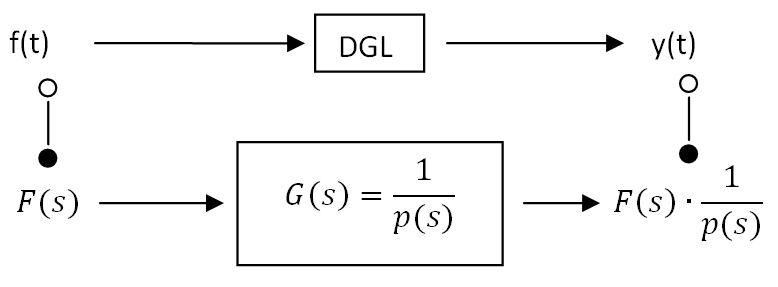
\includegraphics[width=14cm]{../IntTra/bilder/diffgleichungen.png}
				
\newpage

% Diverses
\section{Diverses}
\subsection{Partialbruchzerlegung}
	\[f(x)=\frac{x^2+20x+149}{x^3+4x^2-11x-30} \Rightarrow \; \begin{array}{l}\text{Nenner faktorisieren mit}\\
	\text{Hornerschema, Binom, etc.}\end{array} \Rightarrow
	x^{3}+4x^{2}-11x-30=(x+2)(x^{2}+2x-15)=(x+2)(x+5)(x-3)\] Ansatz:
	\[f(x)=\frac{x^2+20x+149}{x^3+4x^2-11x-30}=\frac{A}{x-3} + \frac{B}{x+2} + \frac{C}{x+5}=
	\frac{A(x+2)(x+5)+B(x-3)(x+5)+C(x-3)(x+2)}{(x-3)(x+2)(x+5)}\]
	Gleichungssystem aufstellen mit beliebigen $x_i$-Werten (am Besten Polstellen oder 0,1,-1 wählen):
	\[\begin{array}{l}x_1=3:\;-9+60+149=A\cdot5\cdot8\;\;\;\Rightarrow A=5\\
	x_2=-2:\;-4-40+149=B(-5)\cdot3\; \Rightarrow B=-7\\
	x_3=-5:\;-25-100+149=C(-8)(-3) \Rightarrow C=1 \end{array} \Rightarrow
	f(x)=\frac{5}{x-3}-\frac{7}{x+2}+\frac{1}{x+5}\] weitere Ansätze für andere
	Typen von Termen: \[f(x)=\frac{5x^2-37x+54}{x^3-6x^2+9x}=\frac{A}{x}+\frac{B}{x-3}+\frac{C}{(x-3)^2}=\frac{A(x-3)^2+Bx(x-3)+Cx}{x(x-3)^2}\]
	\[f(x)=\frac{1,5x}{x^3-6x^2+12x-8}=\frac{A}{x-2}+\frac{B}{(x-2)^2}+\frac{C}{(x-2)^3}=\frac{A(x-2)^2+B(x-2)+C}{(x-2)^3}\]
	\[f(x)=\frac{x^2-1}{x^3+2x^2-2x-12}=\frac{A}{x-2}+\frac{Bx+C}{x^2+4x+6}=\frac{A(x^2+4x+6)+(Bx+C)(x-2)}{(x-2)(x^2+4x+6)}\]
			
\subsection{Hornerschema}
	\begin{minipage}[t]{9cm}
		- Pfeile $\Rightarrow$ Multiplikation\\
		- Zahlen pro Spalte werden addiert\\
		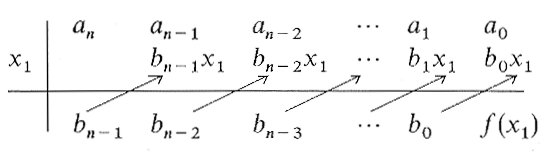
\includegraphics[width=6cm]{./bilder/hornerschema_1.png}\\
		$x_1 \Rightarrow$ Nullstelle (muss erraten werden!!)\\
		oberste Zeile = zu zerlegendes Polynom			
	\end{minipage}
	\begin{minipage}[t]{9cm}
		\textbf{Beispiel:}\\
		$f(x) = x^3-67x-126$\\
		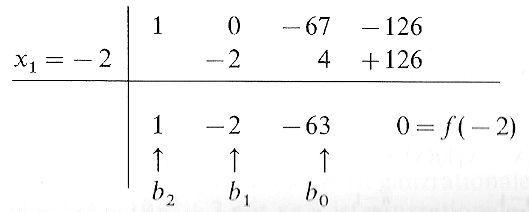
\includegraphics[width=6cm]{./bilder/hornerschema_2.png}\\
		$\Rightarrow f(x) = (x-x_1)(b_2x^2 + b_1x + b_0) = (x+2)(x^2-2x-63)$	
	\end{minipage}

\subsection{Schrittfunktion - unit step}
	\begin{minipage}{10cm}
		$u(t) = \sigma(t) =	\begin{cases}
		  		 0 & \text{für } t < 0 \\
		  		 \frac{1}{2} \text{(praxis)}  \text{ oder undef. (math.)} & \text{für } t = 0 \\
		  		 1 & \text{für } t > 0
		  	\end{cases}
		$
		$\sigma(t) \laplace \frac{1}{j\omega} + \pi\delta(\omega) = \Sigma(\omega)$
	\end{minipage}
	\begin{minipage}{8cm}
		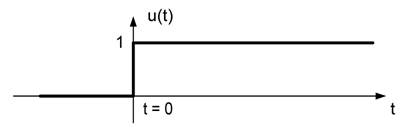
\includegraphics[width=6cm]{./bilder/unitstep.png}
	\end{minipage}

\subsection{Impulsfunktion - dirac delta function}
	\begin{minipage}{10cm}
		$\delta (t)=\begin{cases} 0 & t\ne 0\\\infty & t=0\end{cases} \qquad
		\text{und} \qquad \int\limits_{-\infty}^\infty \delta(t) \, \mathrm dt = 1 $\\
		$$\frac{du(t)}{dt}=\delta(t) \qquad
		\int\limits_{-\infty}^{\infty}\delta(t-t_0)f(t)dt=f(t_0)$$
	\end{minipage}
	\begin{minipage}{8cm}
		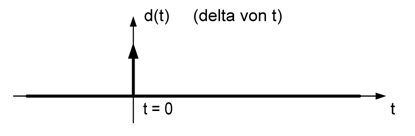
\includegraphics[width=6cm]{./bilder/diracimpulse.png}
	\end{minipage}
\newpage

% Wichtige Formeln
\section{Idiotenseite}
\subsection{Dreiecksformeln}
\begin{tabular}{lll}
	& \parbox{9.5cm}{
		\textbf{Cosinussatz} \\
		$$c^2 = a^2 + b^2 - 2 \cdot a \cdot b \cdot \cos \gamma$$\\
		\textbf{Sinussatz} \\
		$$\frac{a}{\sin \alpha} = \frac{b}{\sin \beta} = \frac{c}{\sin \gamma} = 2r =
		\frac{u}{\pi}$$
		\textbf{Pythagoras beim Sinus}\\
		$$\sin^2(b)+\cos^2(b)=1 \qquad \tan(b)=\frac{\sin(b)}{\cos(b)}$$}
		
	& \parbox{8cm}{
		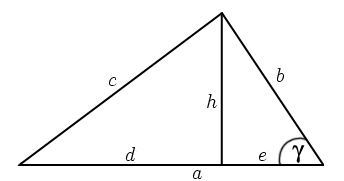
\includegraphics[width=6cm]{./idiotenseite/images/cosinussatz.png}}
\end{tabular}
\begin{center}
	\begin{multicols}{2}
		$\sin \beta = \frac ba =\frac{\text{Gegenkathete}}{\text{Hypotenuse}}$\\
		$\cos \beta = \frac ca =\frac{\text{Ankathete}}{\text{Hypotenuse}}$\\
		$\tan \beta = \frac cb =\frac{\text{Gegenkathete}}{\text{Ankathete}}$\\
		$\cot \beta = \frac cb =\frac{\text{Ankathete}}{\text{Gegenkathete}}$\\
	\end{multicols}
\end{center}

	
\subsection{Funktionswerte für Winkelargumente}
	\begin{minipage}{5cm}	
	\begin{tabular}[c]{|p{0.5cm}|p{0.4cm}||p{0.5cm}|p{0.5cm}|p{0.7cm}|}
	    	\hline
			deg & rad & sin & cos & tan$^-1$\\
			\hline
			0\symbol{23} & 0 & 0 & 1 & 0\\
			\hline
			30\symbol{23} & $\frac{\pi}{6}$ & $\frac{1}{2}$ & $\frac{\sqrt{3}}{2}$ &
			$\frac{1}{\sqrt{3}}$\\
			\hline
			45\symbol{23} & $\frac{\pi}{4}$ & $\frac{\sqrt{2}}{2}$ & $\frac{\sqrt{2}}{2}$
			& 1\\
			\hline
			60\symbol{23} & $\frac{\pi}{3}$ & $\frac{\sqrt{3}}{2}$ & $\frac{1}{2}$ &
			$\sqrt{3}$\\
			\hline			
	\end{tabular} \\
\end{minipage}
\begin{minipage}{14cm}
	\begin{multicols}{3}	
	\begin{tabular}[c]{|p{0.7cm}|p{0.7cm}||p{0.7cm}|p{0.7cm}|}
	    	\hline
			deg & rad & sin & cos\\
			\hline
			90\symbol{23} & $\frac{\pi}{2}$ & 1 & 0\\
			\hline	
			120\symbol{23} & $\frac{2\pi}{3}$ & $\frac{\sqrt{3}}{2}$ & $-\frac{1}{2}$ \\
			\hline
			135\symbol{23} & $\frac{3\pi}{4}$ & $\frac{\sqrt{2}}{2}$ & $-\frac{\sqrt{2}}{2}$\\
			\hline
			150\symbol{23} & $\frac{5\pi}{6}$ & $\frac{1}{2}$ & $-\frac{\sqrt{3}}{2}$\\
			\hline
	\end{tabular} \\
	
	\begin{tabular}[c]{|p{0.7cm}|p{0.7cm}||p{0.7cm}|p{0.7cm}|}
	  	\hline
		deg & rad & sin & cos\\
		\hline
		180\symbol{23} & $\pi$ & 0 & -1\\
		\hline	
		210\symbol{23} & $\frac{7\pi}{6}$ & $-\frac{1}{2}$ & $-\frac{\sqrt{3}}{2}$\\
		\hline
		225\symbol{23} & $\frac{5\pi}{4}$ & $-\frac{\sqrt{2}}{2}$ & $-\frac{\sqrt{2}}{2}$\\
		\hline
		240\symbol{23} & $\frac{4\pi}{3}$ & $-\frac{\sqrt{3}}{2}$ & $-\frac{1}{2}$\\
		\hline
	\end{tabular} \\
	
	\begin{tabular}[c]{|p{0.7cm}|p{0.7cm}||p{0.7cm}|p{0.7cm}|}
    	\hline
		deg & rad & sin & cos\\
		\hline
		270\symbol{23} & $\frac{3\pi}{2}$ & -1 & 0\\
		\hline	
		300\symbol{23} & $\frac{5\pi}{3}$ & $-\frac{\sqrt{3}}{2}$ & $\frac{1}{2}$\\
		\hline
		315\symbol{23} & $\frac{7\pi}{4}$ & $-\frac{\sqrt{2}}{2}$ & $\frac{\sqrt{2}}{2}$\\
		\hline
		330\symbol{23} & $\frac{11\pi}{6}$ & $-\frac{1}{2}$ & $\frac{\sqrt{3}}{2}$\\
		\hline
	\end{tabular}					
\end{multicols}
\end{minipage}

\begin{minipage}{13cm}
	\subsection{Periodizität}
	$\cos(a+k\cdot2\pi)=\cos(a) \qquad \sin(a+k\cdot2\pi)=\sin(a) \qquad
	(k \in \mathbb{Z})$
	\subsection{Quadrantenbeziehungen}
	\begin{tabbing}
    	xxxxxxxxxxxxxxxxxxxxxxxxxxxxxxxxxx \= \kill
	  	$\sin(-a)=-\sin(a)$ \> $\cos(-a)=\cos(a)$\\
		$\sin(\pi - a)=\sin(a)$ \> $\cos(\pi - a)=-\cos(a)$\\
		$\sin(\pi + a)=-\sin(a)$ \> $\cos(\pi +a)=-\cos(a)$\\
		$\sin\left(\frac{\pi}{2}-a \right)=\sin\left(\frac{\pi}{2}+a \right)=\cos(a)$ \>
		$\cos\left(\frac{\pi}{2}-a \right)=-\cos\left(\frac{\pi}{2}+a \right)=\sin(a)$  
    \end{tabbing}
\end{minipage}
\begin{minipage}{5cm}
	

\subsection{Ableitungen}

\begin{tikzpicture}
	[	inner sep = 2mm,
		sin/.style={rectangle,minimum width=1.2cm,minimum height=1cm,rounded corners=5pt,draw=black,top color=green!20!black!50},
		abl/.style={rectangle}
	]
	\node at (1.2,0) (sin1) [sin] {$\sin$};
	\node at (0,-1.2) (cos2) [sin] {$-\cos$};
	\node at (1.2,-2.4) (sin2) [sin] {$-\sin$};
	\node at (2.4,-1.2) (cos1) [sin] {$\cos$};
	
	\draw[thick,black,->] (sin1.east) .. controls +(right:0.6cm) and +(up:0.6cm) ..  (cos1.north)
	node [pos=0.5,above](abl) {$\frac{d}{dx}$};
	\draw[thick,black,->] (cos1.south) .. controls +(down:0.6cm) and +(right:0.6cm) .. (sin2.east)
	node [pos=0.5,below](abl) {$\frac{d}{dx}$};
	\draw[thick,black,->] (sin2.west) .. controls +(left:0.6cm) and +(down:0.6cm) .. (cos2.south)
	node [pos=0.5,below](abl) {$\frac{d}{dx}$};
	\draw[thick,black,->] (cos2.north) .. controls +(up:0.6cm) and +(left:0.6cm) .. (sin1.west)
	node [pos=0.5,above](abl) {$\frac{d}{dx}$};
\end{tikzpicture}
\end{minipage}
\begin{multicols}{2}
	\subsection{Additionstheoreme}
	$\sin(a \pm b)=\sin(a) \cdot \cos(b) \pm \cos(a) \cdot \sin(b)$\\
	$\cos(a \pm b)=\cos(a) \cdot \cos(b) \mp \sin(a) \cdot \sin(b)$\\	
	$\tan(a \pm b)=\dfrac{\tan(a) \pm \tan(b)}{1 \mp \tan(a) \cdot \tan(b)}$
	\columnbreak
	
	\subsection{Doppel- und Halbwinkel}	
	$\sin(2a)=2\sin(a)\cos(a)$\\
	$\cos(2a)=\cos^2(a)-\sin^2(a)=2\cos^2(a)-1=1-2\sin^2(a)$\\
	$\cos^2 \left(\frac{a}{2}\right)=\frac{1+\cos(a)}{2} \qquad
	\sin^2 \left(\dfrac{a}{2}\right)=\frac{1-\cos(a)}{2}$
\end{multicols}
\begin{multicols}{2}
	\subsection{Produkte}
		$\sin(a)\sin(b)=\frac{1}{2}(\cos(a-b)-\cos(a+b))$\\
		$\cos(a)\cos(b)=\frac{1}{2}(\cos(a-b)+\cos(a+b))$\\
		$\sin(a)\cos(b)=\frac{1}{2}(\sin(a-b)+\sin(a+b))$\\
	\subsection{Euler-Formeln} 

	$\sin(x) = \frac{1}{2j} \left(e^{jx} - e^{-jx}\right) \qquad
	\cos(x) = \frac{1}{2} \left(e^{jx} + e^{-jx}\right)$ \\
	$e^{x+jy} = e^x \cdot e^{jy} = e^x \cdot \left(\cos(y) + j\sin(y)\right)$ \\
	$e^{j\pi} = e^{-j\pi} = -1$ \\
	\columnbreak
	
	\subsection{Summe und Differenz}
		$\sin(a)+\sin(b)=2 \cdot \sin \left(\frac{a+b}{2}\right) \cdot
		\cos\left(\frac{a-b}{2}\right)$\\
		$\sin(a)-\sin(b)=2 \cdot \sin \left(\frac{a-b}{2}\right) \cdot
		\cos\left(\frac{a+b}{2}\right)$\\
		$\cos(a)+\cos(b)=2 \cdot \cos \left(\frac{a+b}{2}\right) \cdot
		\cos\left(\frac{a-b}{2}\right)$\\
		$\cos(a)-\cos(b)=-2 \cdot \sin \left(\frac{a+b}{2}\right) \cdot
		\sin\left(\frac{a-b}{2}\right)$\\
		$\tan(a) \pm \tan(b)=\dfrac{\sin(a \pm b)}{\cos(a)\cos(b)}$\\
\end{multicols}

\subsection{Diverses}
\begin{tabbing}
	xxxxxxxxxxxxxxxxxxxxxxxxxxxx \= xxxxxxxxxxxxxxxxxxxxxxxxxxxxxx \= \kill
 	$f'(z) = \lim \limits_{\Delta z \rightarrow 0} \frac{f(z + \Delta z) -
	f(z)}{\Delta z}$ \> $(a + b)^n = \sum_{k=0}^{n} \binom n k a^{n-k} \cdot b^k$ \>
	$(a \pm b)^3 =a^3 \pm  3 a^{2} b + 3 a b^2 \pm b^3 $\\ \\
	$x_{1,2} = \dfrac{-b \pm \sqrt{b^2 - 4ac}}{2a}$ \> $\binom n k = \dfrac{n!}{k!
	\cdot (n-k)!}$ \> $(a \pm b)^4 =a^4 \pm  4 a^{3} b + 6a^2b^2 \pm 4 a b^3 +
	b^4$\\
\end{tabbing}
\subsection{Reihenentwicklungen}
\begin{tabular}{llll}
\textbf{Geometrische Reihe}
	& $\sum\limits_{n=0}^{\infty} x^n$ 
	& $= \dfrac{1}{1-x}$
	& $|x| < 1$ \\
	
	& $\sum\limits_{k=0}^{\infty} k \, x^k$ & $= x \sum\limits_{k=1}^{\infty} k \,
	x^{k-1} = \dfrac{x}{(1-x)^2} $ 
	& $x \neq 1$ \\
\textbf{Binominalreihe} 
	& $\sum\limits_{n=0}^\infty \binom{\alpha}{n} x^n $ &$= (1+x)^\alpha$
	& $x \in (-1,1)$ \\
\textbf{E-Funktion}
	& $\sum\limits_{k = 0}^{\infty} \dfrac{x^k}{k!}$ &$ = e^x$
	& 
\end{tabular}

\subsection{Kurven}
\begin{multicols}{4}
\subsubsection{e-Funktion}
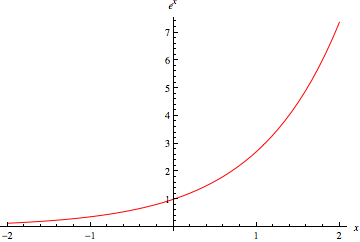
\includegraphics[width=4.5cm]{idiotenseite/images/Exp.png}
\subsubsection{Sinus-Funktion}
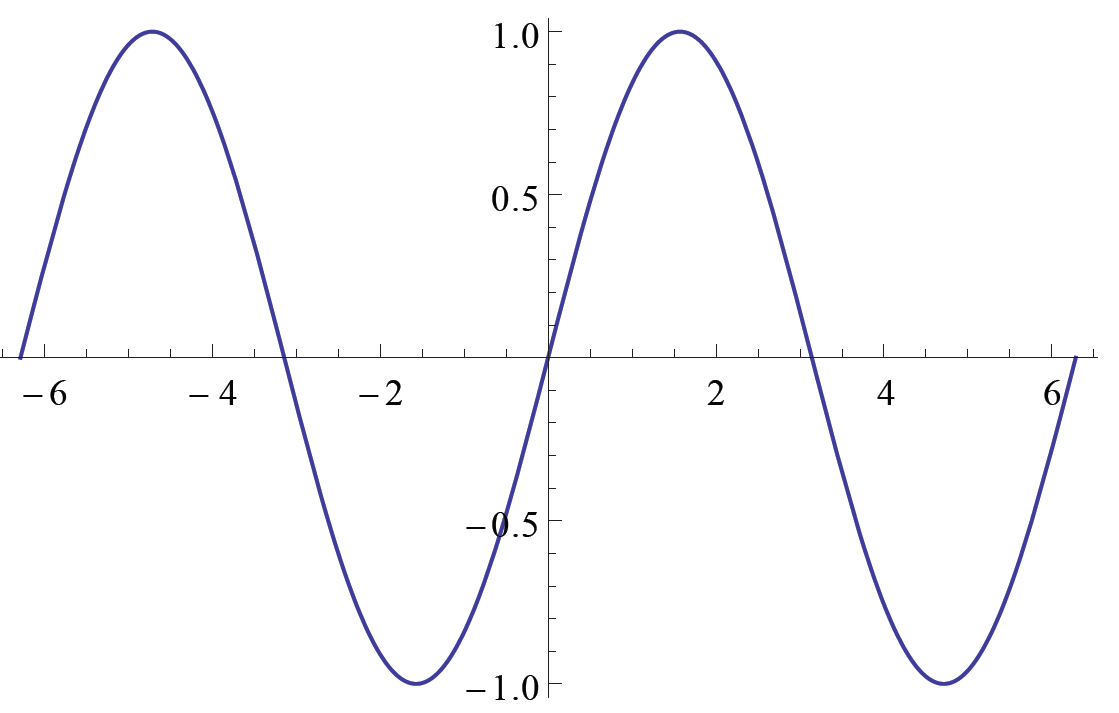
\includegraphics[width=4.5cm]{idiotenseite/images/sin.png}
\subsubsection{Cosinus-Funktion}
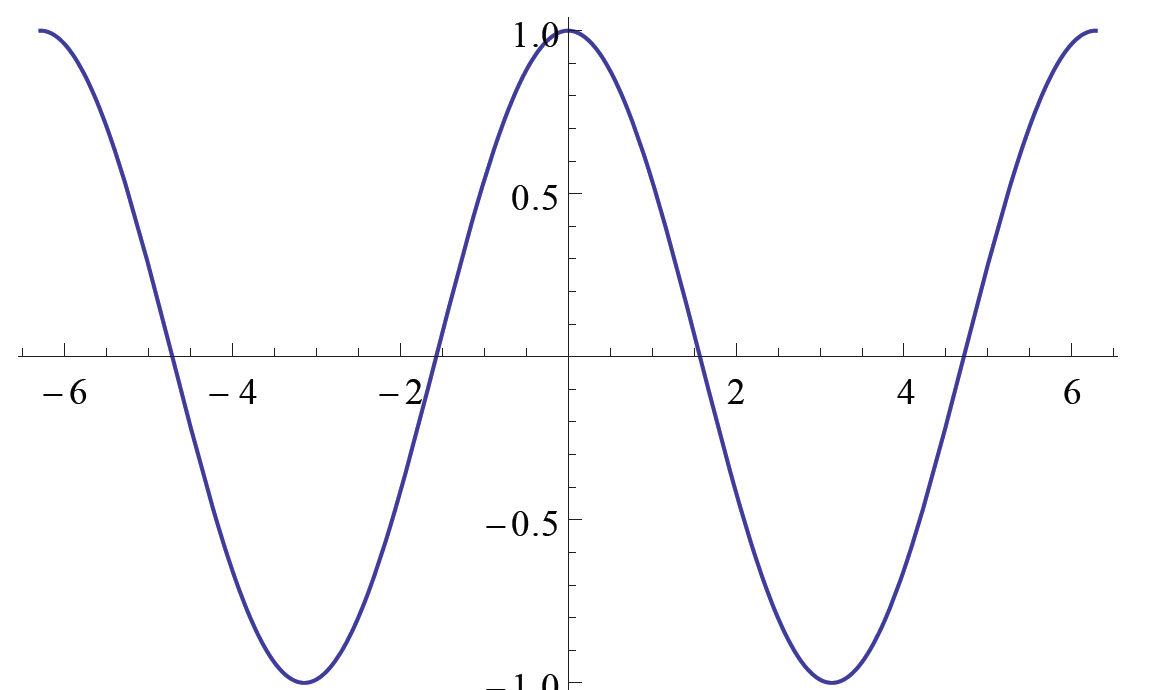
\includegraphics[width=4.5cm]{idiotenseite/images/cos.png}
\subsubsection{Tangens-Funktion}
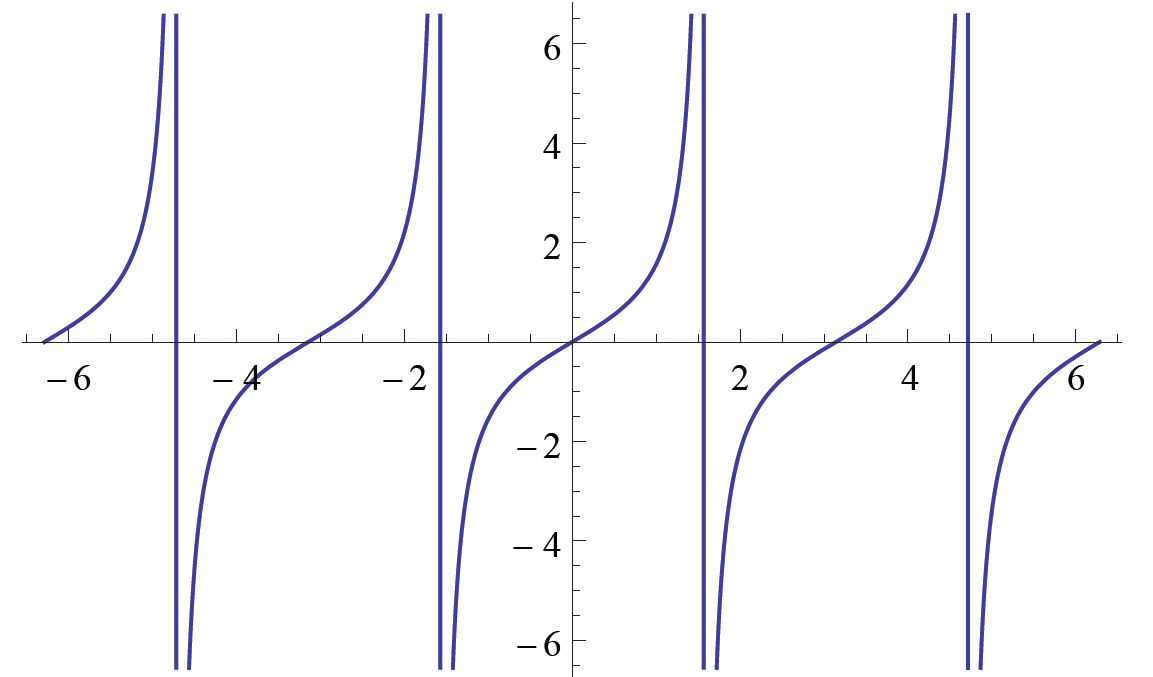
\includegraphics[width=4.5cm]{idiotenseite/images/tan.png}
\end{multicols}
%\subsection{Idiotenformel}
Wenn ihr wissen wollt was die Formel besagt dann kauft euch doch nächstes mal
die Pro Version der Formelsammlung. Arme Schmarotzer und asoziale Personen
dürfen gerne lange darüber Rätseln was das hier soll. Aber wer zu doof ist eine
Formelsammlung ehrlich zu erwerben hat sowieso keine Chance. Haha.\\
$\frac{1}{F_{Siedlungsfl\ddot ache}}\cdot\int\limits_{\vec{x} \in
Siedlungsfl\ddot ache} \frac{1}{\int\limits_{\vec{y}\in Siedlungsfl\ddot ache\ und \left|\vec{x}-\vec{y} \right|<BH}\vec{dy}} \int\limits_{\vec{y}\in Siedlungsfl\ddot ache\ und \left|\vec{x}-\vec{y} \right|<BH} \sqrt{\frac{2\cdot\left|\vec{x}-\vec{y}\right|}{1m}+1}-1\vec{dy}\vec{dx}\frac{DSE}{m^2}$

\subsection{SI-Vorsätze}

\begin{multicols}{2}
\begin{tabular}{|l|l|l|l|}
\hline
\textbf{Symbol}	& \textbf{Name} & \textbf{Wert} & \textbf{Binär} \\
\hline
da	& Deka 	& $10^1$ & \\
\hline
h	& Hekto & $10^2$ & \\ 
\hline
k	& Kilo	& $10^3$ & $2^{10} = 1024$ \\
\hline
M	& Mega	& $10^6$ & $2^{20}$\\
\hline
G	& Giga  & $10^9$ & $2^{30}$\\
\hline
T	& Tera	& $10^{12}$ & $2^{40}$ \\
\hline
P	& Peta	& $10^{15}$ & $2^{50}$\\
\hline
\end{tabular}

\columnbreak

\begin{tabular}{|l|l|l|}
\hline
\textbf{Symbol}	& \textbf{Name} & \textbf{Wert} \\
\hline
d	& Dezi	& $10^{-1}$ \\
\hline
c	& Centi	& $10^{-2}$ \\ 
\hline
m	& Milli	& $10^{-3}$ \\
\hline
y, $\mu$ & Mikro & $10^{-6}$ \\
\hline
n	& Nano	& $10^{-9}$ \\
\hline
p	& Piko	& $10^{-12}$ \\
\hline
f	& Femto & $10^{-15}$ \\
\hline
\end{tabular}
\end{multicols}
\subsection{GrichischesAlphabet}
\begin{multicols}{2}
	\subsubsection{klein}
	\begin{tabular}{ |l|l|l|l|l|l|l|l|}
		\hline
		$\alpha$&Alpha&$\theta$&Theta&o&o&$\tau$&Tau\\
		\hline
		$\beta$&Beta&$\vartheta$&Theta&$\pi$&Pi&$\upsilon$&Ypsilon\\
		\hline
		$\gamma$&Gamma&$\gamma$&Gamma&$\varpi$&Pi&$\phi$&Phi\\
		\hline
		$\delta$&Delta&$\kappa$&Kappa&$\rho$&Roh&$\varphi$&Phi\\
		\hline
		$\epsilon$&Epsilon&$\lambda$&Lambda&$\varrho$&Roh&$\chi$&Chi\\
		\hline
		$\varepsilon$&Epsilon&$\mu$&Mu&$\sigma$&Sigma&$\psi$&Psi\\
		\hline
		$\zeta$&Zeta&$\nu$&Nu&$\varsigma$&Sigma&$\omega$&Omega\\
		\hline
		$\eta$&Eta&$\xi$&Xi&&&&\\
		\hline
	\end{tabular}
	\columnbreak
	
	\subsubsection{gross}
	\begin{tabular}{|l|l|l|l|l|l|l|l|}
		\hline
		$\Gamma$&Gamma&$\Lambda$&Lambda&$\Sigma$&Sigma&$\Psi$&Psi\\
		\hline
		$\Delta$&Delta&$\Xi$&Xi&$\Upsilon$&Ypsilon&$\Omega$&Omega\\
		\hline
		$\Theta$&Theta&$\Pi$&Pi&$\Phi$&Phi&&\\
		\hline
	\end{tabular}
\end{multicols}
\begin{sidewaystable}
\subsection{Einige unbestimmte Integrale\formelbuch{1074}}
\label{unbestimmte_integrale}
\begin{tabular}{|p{12cm}|p{13cm}|}
  \hline
  
    $ \int dx=x+C $ &
     $ \int{x^\alpha}dx=\frac{x^{\alpha+1}}{\alpha+1}+C,\ x \epsilon \mathbb
    R ^+,\ \alpha \epsilon \mathbb R \backslash \{ -1 \} $ \\\hline
     $ \int{\frac{1}{x}}dx=\ln \left| x \right| + C,\ x\neq0 $ &
     $ \int{e^x}dx=e^x+C $ \\\hline
     $ \int{a^x}dx=\frac{a^x}{\ln{a}}+C,\ a \epsilon \mathbb 
    R^+\backslash\{1\} $ &
     $ \int{ \sin{x}} dx = -\cos{x} + C $ \\\hline
     $ \int{\cos{x}} dx = \sin{x} + C $ &
     $ \int{\frac{dx}{\sin^2x}}=-\cot{x}+C,\ x\neq k\pi\ \mathrm{mit}\ k
    \epsilon \mathbb Z $ \\\hline
     $ \int{\frac{dx}{\cos^2x}}=\tan{x}+C,\ x\neq\frac{\pi}{2}+k\pi\
    \mathrm{mit} k \epsilon \mathbb Z $ & 
    
    %10. :
     $ \int{\sinh{x}}dx = \cosh{x}+C $ \\ \hline
     $ \int{\cosh{x}}dx = \sinh{x}+C $ &
     $ \int{\frac{dx}{\sinh^2x}}=-\coth{x}+C,\ x\neq0 $ \\\hline
     $ \int{\frac{dx}{\cosh^2x}}=\tanh{x}+C $ &
     $ \int{\frac{dx}{ax+b}} = \frac{1}{a}\ln \left|ax + b\right| + C,\
    a\neq 0,x\neq-\frac{b}{a} $ \\\hline
     $ \int{\frac{dx}{a^2x^2+b^2}}=\frac{1}{ab}\arctan{\frac{a}{b}x}+C,\
    a\neq0,\ b\neq0 $ &
     $
    \int{\frac{dx}{a^2x^2-b^2}}=\frac{1}{2ab}\ln{\left|\frac{ax-b}{ax+b}\right|}+C,\
    a\neq0,\ b\neq0,\ x\neq\frac{b}{a},\ x\neq-\frac{b}{a} $ \\\hline
     $
    \int{\sqrt{a^2x^2+b^2}}dx=\frac{x}{2}\sqrt{a^2x^2+b^2}+\frac{b^2}{2a}\ln{(ax+\sqrt{a^2x^2+b^2})}+C,\
    a\neq0,\ b\neq0 $ &
     $
    \int{\sqrt{a^2x^2-b^2}}dx=\frac{x}{2}\sqrt{a^2x^2-b^2}-\frac{b^2}{2a}\ln\left|ax+\sqrt{a^2x^2-b^2}\right|+C,\
    a\neq0,\ b\neq0,a^2x^2\geqq b^2$ \\\hline
     $
    \int\sqrt{b^2-a^2x^2}dx=\frac{x}{2}\sqrt{b^2-a^2x^2}+\frac{b^2}{2a}\arcsin\frac{a}{b}x+C,\
    a\neq0,\ b\neq0,\ a^2x^2\leqq b^2 $ &
    %20.:
     $
    \int\frac{dx}{\sqrt{a^2x^2-b^2}}=\frac{1}{a}\ln(ax+\sqrt{a^2x^2+b^2})+C,\
    a\neq0,\ b\neq0 $ \\\hline
     $
    \int\frac{dx}{\sqrt{a^2x^2-b^2}}=\frac{1}{a}\ln\left|ax+\sqrt{a^2x^2-b^2}\right|+C,\
    a\neq0,\ b\neq0,\ a^2x^2>b^2 $ &
     $ \int\frac{dx}{\sqrt{b^2-a^2x^2}}=\frac{1}{a}\arcsin\frac{a}{b}x+C,\
    a\neq0,\ b\neq0,\ a^2x^2<b^2 $ \\\hline
     Die Integrale $\int\frac{dx}{X}, \int\sqrt{X}dx,
    \int\frac{dx}{\sqrt{X}}$ mit $X=ax^2+2bx+c,\ a\neq0 $ werden durch 
    die Umformung $X=a(x+\frac{b}{a})^2+(c-\frac{b^2}{a}) $ und die
    Substitution $ t=x+\frac{b}{a} $ in die oberen 4 Zeilen
    transformiert. & $ \int\frac{xdx}{X}=\frac{1}{2a}\ln\left|X\right|-\frac{b}{a}\int\frac{dx}{X},\
    a\neq0,\ X=ax^2+2bx+c $ \\\hline
     $ \int\sin^2axdx=\frac{x}{2}-\frac{1}{4a}\cdot\sin2ax+C,\ a\neq0 $ &
     $ \int\cos^2axdx=\frac{x}{2}+\frac{1}{4a}\cdot\sin2ax+C,\ a\neq0 $ \\\hline
     $ \int\sin^naxdx=-\frac{sin^{n-1}ax\cdot\cos
    ax}{na}+\frac{n-1}{n}\int\sin^{n-2}axdx,\ n \epsilon \mathbb N,\ a\neq0 $ &
     $ \int\cos^naxdx=\frac{\cos^{n-1}ax\cdot\sin
    ax}{na}+\frac{n-1}{n}\int\cos^{n-2}axdx,\ n\epsilon \mathbb N,\ a\neq0 $
    \\\hline
     $ \int\frac{dx}{\sin ax} =
    \frac{1}{a}\ln\left|\tan\frac{ax}{2}\right|+C,\ a\neq0,\ x\neq
    k\frac{\pi}{a}\ \mathrm{mit}\ k\epsilon\mathbb Z$ &
    %30.:
     $ \int\frac{dx}{\cos
    ax}=\frac{1}{a}\ln\left|\tan(\frac{ax}{2}+\frac{\pi}{4})\right|+C,\ a\neq0,\
    x\neq\frac{\pi}{2a}+k\frac{\pi}{a}\ \mathrm{mit}\ k\epsilon\mathbb Z $
    \\\hline
     $\int\tan axdx=-\frac{1}{a}\ln\left|\cos ax\right|+C,\ a\neq0,\
    x\neq\frac{\pi}{2a}+k\frac{\pi}{a} \mathrm{mit}\ k\epsilon\mathbb Z$ &
     $\int\cot axdx=\frac{1}{a}\ln\left|\sin ax\right|+C,\ a\neq0,\ x\neq
    k\frac{\pi}{a} \mathrm{mit} k\epsilon\mathbb Z $ \\ \hline
     $ \int x^n\sin axdx=-\frac{x^n}{a}\cos ax+\frac{n}{a}\int x^{n-1}\cos
    axdx,\ n\epsilon\mathbb N,\ a\neq0 $ &
    $ \int x^n\cos axdx=\frac{x^n}{a}\sin ax-\frac{n}{a}\int x^{n-1}\sin
    axdx,\ n\epsilon\mathbb N,\ a\neq0 $ \\ \hline
     $ \int x^ne^{ax}dx=\frac{1}{a}x^ne^{ax}-\frac{n}{a}\int
    x^{n-1}e^{ax}dx,\ n\epsilon\mathbb N,\ a\neq0 $ &
     $ \int e^{ax}\sin bxdx=\frac{e^{ax}}{a^2+b^2}(a\sin bx-b\cos bx)+C,\
    a\neq0,\ b\neq0 $  \\ \hline
     $ \int e^{ax}\cos bxdx=\frac{e^{ax}}{a^2+b^2}(a\cos bx + b\sin bx)+C,\
    a\neq0,\ b\neq0 $ &
     $ \int\ln x dx = x(\ln x-1)+C,\ x\epsilon\mathbb R^+ $ \\ \hline
     $ \int x^\alpha \cdot \ln xdx =
    \frac{x^{\alpha+1}}{(\alpha+1)^2}\lbrack(\alpha+1)\ln x-1\rbrack + C,\
    x\epsilon\mathbb R^+,\ \alpha\epsilon\mathbb R\backslash\{-1\} $ & \\ \hline
    %FF1 Seite 496
    
\end{tabular}
\end{sidewaystable}
%\begin{sidewaystable}
\subsection{Ableitungen elementarer Funktionen\formelbuch{436}}
\label{unbestimmte_integrale}
\renewcommand{\arraystretchOriginal}{2.5}
\begin{tabular}{|l|l||l|l|}
  \hline
  \textbf{Funktion} & \textbf{Ableitung} & \textbf{Funktion} &
  \textbf{Ableitung}\\\hline
  $C$ (Konstante) & 0 & $\sec x$ & $\dfrac{\sin x}{\cos^2 x}$ \\
  $x$ & 1 & $\sec^{-1} x$ & $\dfrac{-\cos x}{\sin^2 x}$\\
  $x^n$ ($n\in\mathbb{R}$) & $nx^{n-1}$ & $\arcsin x \quad (|x| < 1)$ &
  $\dfrac{1}{\sqrt{1-x^2}}$\\
  $\dfrac{1}{x}$ & $-\dfrac{1}{x^2}$ & $\arccos x \quad (|x| < 1)$ &
  $-\dfrac{1}{\sqrt{1-x^2}}$\\
  $\dfrac{1}{x^n}$ & $-\dfrac{n}{x^{n+1}}$ & $\arctan x$ & $\dfrac{1}{1+x^2}$\\
  $\sqrt{x}$ & $\dfrac{1}{2\sqrt{x}}$ & arccot $x$ & $-\dfrac{1}{1+x^2}$\\
  $\sqrt[n]{x}\quad (n\in\mathbb{R}, n \neq 0, x > 0)$ &
  $\dfrac{1}{n\sqrt[n]{x^{n-1}}}$ & arcsec $x$ & $\dfrac{1}{x\sqrt{x^2-1}}$\\
  $\mathrm{e}^x$ & $\mathrm{e}^x$ & arcossec $x$ & $-\dfrac{1}{x\sqrt{x^2-1}}$\\
  $\mathrm{e}^{bx}\quad (b\in\mathbb{R})$ & $b\mathrm{e}^{bx}$ & $\sinh x$ &
  $\cosh x$\\
  $a^x\quad (a > 0)$ & $a^x\ln a$ & $\cosh x$ & $\sinh x$\\
  $a^{bx}\quad (b\in\mathbb{R}, a > 0)$ & $ba^{bx}\ln a$ & $\tanh x$ &
  $\dfrac{1}{\cosh^2 x}$\\
  $\ln x$ & $\dfrac{1}{x}$ & $\coth x \quad(x \neq 0)$ & $-\dfrac{1}{\sinh^2 x}$\\
  $\log_a{x} \quad (a > 0, a \neq 1, x > 0)$ &
  $\dfrac{1}{x}\log_a{\mathrm{e}}=\dfrac{1}{x\ln a}$ & Arsinh $x$ &
  $\dfrac{1}{\sqrt{1+x^2}}$\\
  $\lg x \quad (x > 0)$ & $\dfrac{1}{x}\lg \mathrm{e}\approx \dfrac{0.4343}{x}$
  & Arcosh $x \quad (x > 1)$ & $\dfrac{1}{\sqrt{x^2-1}}$\\
  $\sin x$ & $\cos x$ & Artanh $x \quad (|x| < 1)$ & $\dfrac{1}{1-x^2}$\\
  $\cos x$ & $-\sin x$ & Arcoth $x \quad (|x| > 1)$ & $-\dfrac{1}{x^2-1}$\\
  $\tan x \quad (x\neq(2k+1)\dfrac{\pi}{2}, k\in\mathbb{Z})$ & $\dfrac{1}{\cos^2
  x}=\sec^2 x$ & $[f(x)]^n \quad (n\in\mathbb{R})$ & $n[f(x)]^{n-1}f'(x)$\\
  $\cot x \quad (x\neq k\pi, k\in\mathbb{Z})$ & $\dfrac{-1}{\sin^2 x}=-cosec^2x$ & $\ln f(x) \quad (f(x)> 0)$ & $\dfrac{f'(x)}{f(x)}$\\
  \hline
\end{tabular}
\renewcommand{\arraystretchOriginal}{1.5}
%\end{sidewaystable}



\newpage

% Integraltabelle
\section{Integralrechnung}
Partielle Integration: $\int u(x) v'(x) dx = u(x)v(x) - \int u'(x) v(x) dx$

\subsection{Einige wichtige Integrale}
  	\renewcommand{\arraystretch}{2}
	\begin{tabular}{|l|l|}
    	\hline
    	$\int \sin(x)dx=-\cos(x)$ & $\int \sin(a+bx)dx=-\frac1b \cos(a+bx)$\\
    	\hline
	  	$\int \sin^2(x)dx=-\frac14 \sin(2x)+\frac x2$ 
    	& $\int
    	e^{ax+c}\sin(bx+d)dx=\frac{e^{ax+c}}{a^2+b^2}(a\sin(bx+d)-b\cos(bx+d))$\\
    	\hline
    	$\int \cos(x)dx=\sin(x)$ & $\int \cos(a+bx)dx=\frac1b \sin(a+bx)$\\
    	\hline
	  	$\int \cos^2(x)dx=\frac14 \sin(2x)+\frac x2$ 
    	& $\int
    	e^{ax+c}\cos(bx+d)dx=\frac{e^{ax+c}}{a^2+b^2}(a\cos(bx+d)+b\sin(bx+d))$\\
    	\hline
    	$\int e^x dx=e^x$ & $\int e^{ax}dx=\frac1a e^{ax}$\\
    	\hline
    	$\int xe^{ax}dx=\frac{1}{a^2} e^{ax}(ax-1)$ & $\int x^2 e^{ax} dx =
    	e^{ax}\left( \frac{x^2}{a} - \frac{2x}{a^2} + \frac{2}{a^3}\right)$ \\
    	\hline
    	$\int x^n e^{ax} dx = \frac{1}{a} x^n e^{ax} - \frac{n}{a} \int x^{n-1}
    	e^{ax} dx$ & \\
    	\hline
    \end{tabular}

\section{Differentialrechnung}
\subsection{Einige wichtige Differentiale}
	\begin{tabular}{|l|l||l|l|}
    	\hline
    	\textbf{Funktion} & \textbf{Ableitung} & \textbf{Funktion} &
    	\textbf{Ableitung}\\
    	\hline
    	\hline
    	$C \text{ (Konstante)}$ & $0$ & $x$ & $1$\\
    	\hline
    	$x^n$ & $nx^{n-1}$ & $\frac1x$ & $-\frac{1}{x^2}$\\
    	\hline
    	$\sqrt{x}$ & $\frac{1}{2\sqrt{x}}$ & $e^x$ & $e^x$\\
    	\hline
    	$e^{bx}$ & $be^{bx}$ & $a^x$ & $a^x \ln(a)$\\
    	\hline
    	$\ln(x)$ & $\frac1x$ & $\sin(x)$ & $\cos(x)$\\
    	\hline
    	$\cos(x)$ & $-\sin(x)$ & $\ln[f(x)]$ & $\frac{f^{'}(x)}{f(x)}$\\
    	\hline
		
    \end{tabular}
  	\renewcommand{\arraystretch}{1}
\newpage

% Riisä Tricks
\section{Riisä Tricks und Merksätze}
\begin{itemize}
  \item $H(s)$ = UTF = Laplacetransformierte der Impulsantwort ($y_\delta(t)$)
  \item $H(j \omega)$ = Frequenzgang = UTF auf imaginärer Achse
  \item $y_\sigma(t) = \int\limits_0^t y_\delta(u)du$
  \item $\left| \frac{ja + b}{a^2 + b^2} \right| = \sqrt{\frac{1}{a^2 + b^2}}$
  \item Dirac-Funktion: $s(t)\delta(t-t_0) = s(t_0)\delta(t-t_0)$
  \item Antwort eines LTI-Systems auf eine harmonisches Schwingung mit Frequenz $\omega \Rightarrow$ harmonische
  Schwingung mit gleicher Frequenz aber anderer Aplitude und Phase ($\mathcal{L}\{e^{j \omega t}\} = H(\omega) \cdot
  e^{j \omega t}$)
  \item $H(\omega)$ = komplexwertige Funktion der Frequenz $\omega$, die für jede Frequenz $\omega$ die
  Änderung von Amplitude und Phase durch das System speichert = Frequenzgang = Antwort auf harmonische Schwingung
  beliebiger Frequenz
\end{itemize}
\end{document}